% Chapter 4

\chapter{Problème 2D et percussion des floes} % 5th chapter title

\label{Chapter4} % For referencing the chapter elsewhere, use \ref{Chapter5} 

%1----------------------------------------------------------------------------------------



Dans cette section, nous étudierons le floe de glace en deux dimensions (2D). Nous reprendrons le même cheminement qu'en 1D. En d'autres termes, nous partirons de l'approche par réseau de ressort introduite par Balasoiu pour modéliser dans un premier temps le déplacement d'un floe de glace contenant juste trois n\oe{}uds (masses); ensuite nous modéliserons la percussion inélastique sans rebond des n\oe{}uds après choc.






%2----------------------------------------------------------------------------------------

\section{Développement d'un modèle de déplacement des n\oe{}uds}








Étudions le comportement d'un floe de glace 2D modélisé par un réseau de ressorts (3 ressort, 3 dispositifs viseux, et 3 n\oe{}uds) (voir \cref{fig:deplacement2d}).
\begin{figure}[!h]
    \centering
    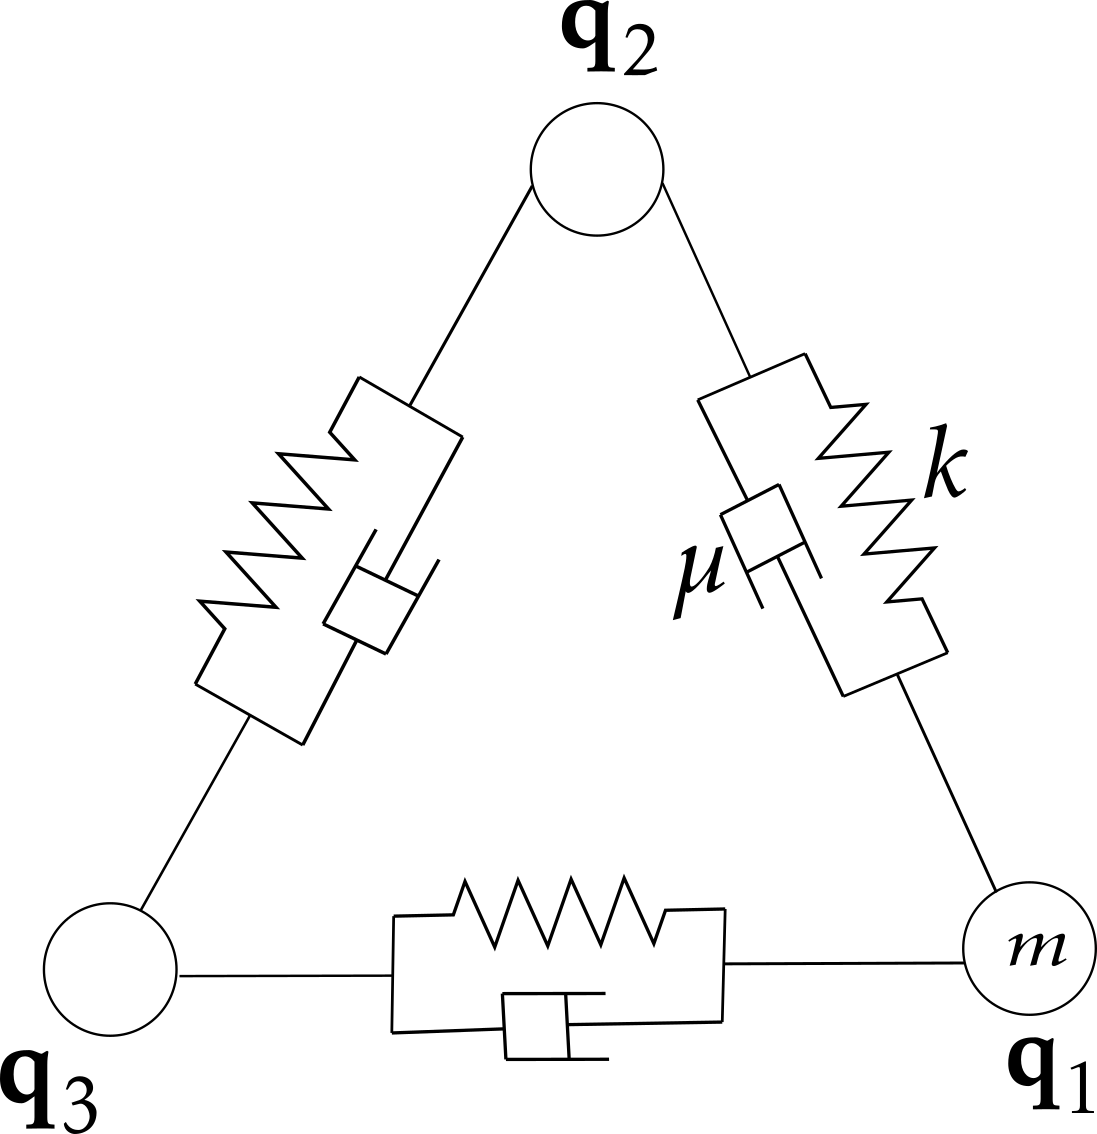
\includegraphics[width=0.3\textwidth]{Deplacement2D-1.png}
    \caption{Floe de glace 2D modélisé par un réseau de ressorts. Le floe est isolé de toutes forces extérieures. Tous les n\oe{}uds du réseau ont la même masse $m$, tous les ressorts on la même raideur $k$, et tous les dispositifs visqueux ont la même viscosité $\mu$.}
    \label{fig:deplacement2d}
\end{figure}


\noindent Comme nous l'avons présenté aux \cref{eq:F0,eq:e}, le système de la \cref{fig:deplacement2d} est régi par l' équation:
\begin{align} \label{eq:eprime2}
    \forall i \in \mathbb{Z}/3\mathbb{Z}, \quad m \ddot{\bvec{q}}_i = \sum_{j=i+1}^{i+2}C_{ij} \left[  k \left( \Vert \bvec{q}_j - \bvec{q}_i \Vert - L_{ij} \right) \bvec{u}_{ij} - \mu \left\langle \bvec{\dot{q}}_j - \bvec{\dot{q}}_i, \, \bvec{u}_{ij}  \right\rangle  \bvec{u}_{ij}  \right]  , 
\end{align}
où $L_{ij}$ représente la longueur au repos du ressort entre les n\oe{}uds $i$ et $j$, et $C_{ij}$ indique si les n\oe{}uds $i$ et $j$ sont connectés ou non (pour ce modèle 2D simple, $C_{ij} = 1 \, \forall 0 \leq i,j \leq 2$). Le vecteur unitaire $\bvec{u}_{ij}$ vaut:
$$
\bvec{u}_{ij} = \frac{\bvec{q}_j - \bvec{q}_i}{\Vert \bvec{q}_j - \bvec{q}_i \Vert}.
$$


\paragraph{Simulation par un schéma d'Euler explicite.}

On discrétise par un schéma de différences finies avec $N+1$ pas de temps, et pour un temps de simulations $T$:
$$
\forall i \in \mathbb{Z}/3\mathbb{Z}, \, \forall n \in [\![ 0,N ]\!], \quad  t^n = n\Delta t = n\frac{T}{N}, \quad \bvec{q}_i(t^n) \approx \bvec{q}_i^n.
$$
L'\cref{eq:eprime2} devient:
$$
m\frac{\bvec{q}_{i}^{n+1}-2\bvec{q}_{i}^{n}+\bvec{q}_{i}^{n-1}}{\Delta t^2} = \sum_{j=i+1}^{i+2}C_{ij}\left[ k \left( \Vert \bvec{q}_j^n - \bvec{q}_i^n \Vert - L_{ij} \right) \bvec{u}_{ij} - \mu \left\langle \frac{\bvec{q}_{j}^{n}-\bvec{q}_{j}^{n-1}}{\Delta t} - \frac{\bvec{q}_{i}^{n}-\bvec{q}_{i}^{n-1}}{\Delta t}, \, \bvec{u}_{ij} \right\rangle  \bvec{u}_{ij}  \right],
$$
soit encore:
\begin{align} \label{eq:systeme2D}
    \bvec{q}_{i}^{n+1} = 2\bvec{q}_{i}^{n}-\bvec{q}_{i}^{n-1} + \frac{\Delta t^2}{m} \sum_{j=i+1}^{i+2}C_{ij}\left[ k \left( \Vert \bvec{q}_j^n - \bvec{q}_i^n \Vert - L_{ij} \right) \bvec{u}_{ij} - \frac{\mu}{\Delta t} \left\langle \bvec{q}_{j}^{n}-\bvec{q}_{j}^{n-1} - \bvec{q}_{i}^{n}+\bvec{q}_{i}^{n-1}, \, \bvec{u}_{ij} \right\rangle  \bvec{u}_{ij}  \right].
\end{align}
La simulation de ce modèle par un schéma d'Euler explicite à pas constant sur un intervalle de temps faible ($T = 4$) est présentée à la \cref{fig:PlotDeplacement2D1Conv}, ainsi que les positions des n\oe{}uds au début et à la fin de la simulation. La simulation à la \cref{fig:PlotDeplacement2D1NonConv} permet d'observer le problème avec ce même schéma à quelques différences près (i.e. $T = 10$).


\begin{figure}[!h]
    \begin{subfigure}[b]{0.7\textwidth}
        \centering
        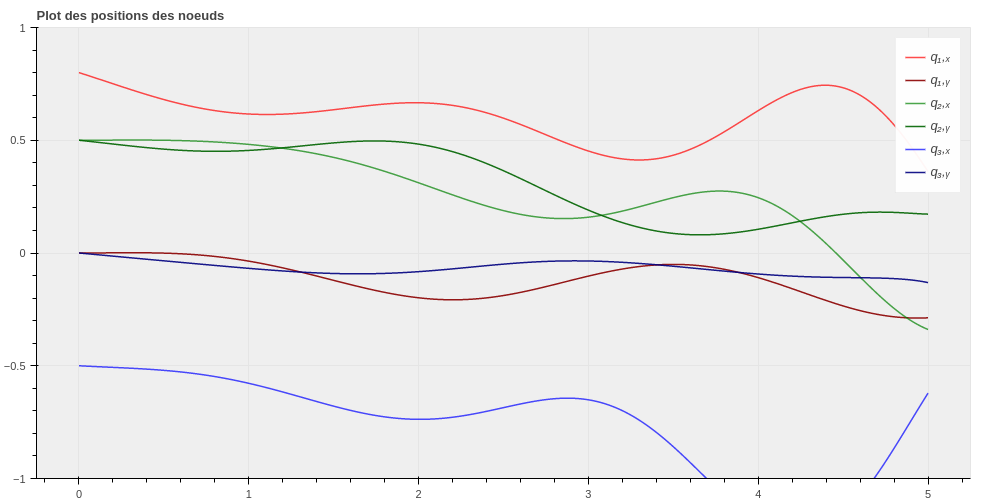
\includegraphics[width=\textwidth]{PlotDeplacement2D-1-Conv.png}
        \caption{Simulation des positions des n\oe{}uds.}
        \label{fig:dep}
    \end{subfigure}
%     \hfill
    \begin{subfigure}[b]{0.7\textwidth}
        \centering
        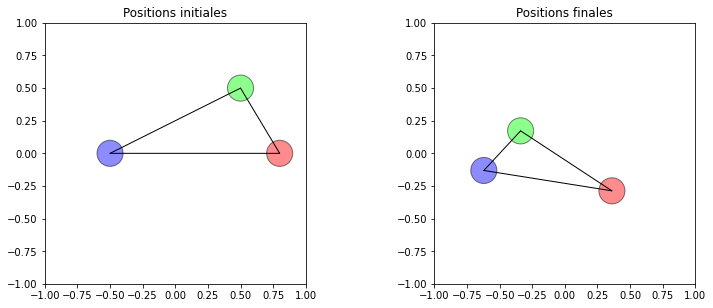
\includegraphics[width=\textwidth]{PositionInitFinales.png}
        \caption{Illustration des positions initiales et finales des n\oe{}uds.}
        \label{fig:pos}
    \end{subfigure}
    \caption{Simulation du système \ref{eq:systeme2D} par un schéma d'Euler explicite avec $T = 4$ lorsqu'\textit{un des n\oe{}uds est fixé} (le n\oe{}ud rouge). La couleur rouge représente le n\oe{}ud $\bvec{q}_1$, le vert le n\oe{}ud $\bvec{q}_2$, le blue le $\bvec{q}_3$. Les paramètres utilisés ici sont les suivants: $m=6.2$, $k=23.3$, $\mu=3$; à l'instant initiale, les trois n\oe{}uds perturbés avec des vitesses d'intensité respectives $v_1=0.3$, $v_2=0.1$, et $v_3=0.1$. Par rapport à l'axe des abscisses, ces vitesses sont orientées respectivement de $\theta_1=180^\circ$, $\theta_2=270^\circ$, et $\theta_3=240^\circ$ (voir \texttt{code/simu2D/Deplacement2D-1.ipynb}).}
    \label{fig:PlotDeplacement2D1Conv}
\end{figure}


\begin{figure}[!h]
    \centering
    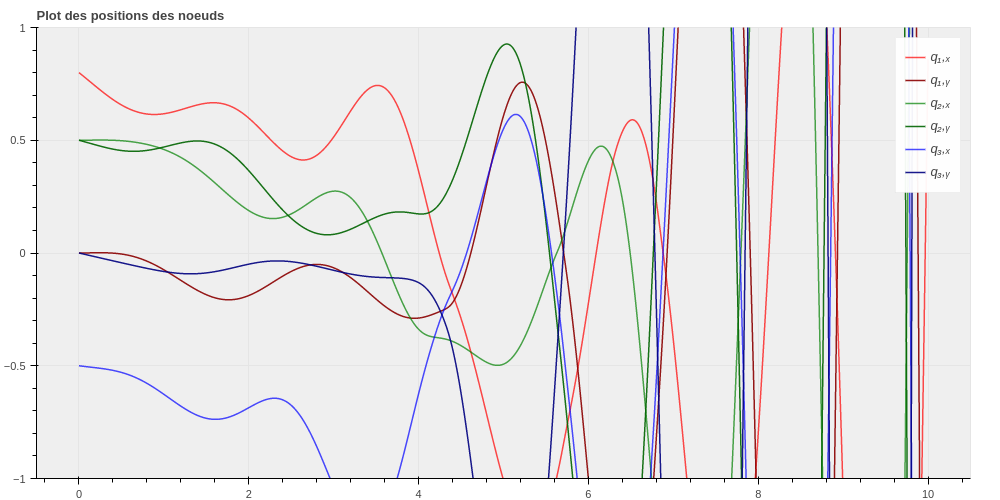
\includegraphics[width=0.7\textwidth]{PlotDeplacement2D-1-NonConv.png}
    \caption{Simulation du système \ref{eq:systeme2D} par un schéma d'Euler explicite avec $T = 10$ lorsqu'\textit{aucun des n\oe{}uds n'est fixé}. Cette figure utilise les mêmes paramètres que la \cref{fig:PlotDeplacement2D1Conv}. On observe ici une divergence complète du système (voir \texttt{code/simu2D/Deplacement2D-2.ipynb}).}
    \label{fig:PlotDeplacement2D1NonConv}
\end{figure}

Les \cref{fig:PlotDeplacement2D1Conv,fig:PlotDeplacement2D1NonConv} sembleraient indiquer que le schéma d'Euler explicite (peu importe son pas de temps), n'est pas adapté à ce problème. On se pose également la question de savoir si la non-stabilité est due au schéma utilisé. En réalité, Balasoiu \parencite{balasoiu2020halthesis} a effectué des simulations similaires avec un schéma symplectique et a aussi dû fixer certains n\oe{}uds pour avoir la stabilité. Nous étudierons donc d'autres alternatives. 

 
\paragraph{Simulation à l'aide des fonctions de la librairie Scipy.} À travers ses fonction telle que \texttt{odeint} et $\verb|solve_ivp|$, \texttt{Scipy} offre une solution robuste et élégante pour simuler les systèmes d'ODE de la forme $Y' = AY$. Avec \texttt{Scipy}, nous résolvons numériquement nos EDO à l'ordre \href{https://docs.scipy.org/doc/scipy/reference/generated/scipy.integrate.solve_ivp.html}{RK45}. Autrement dit, l'erreur est contrôlée par un schéma de Runke-Kutta à l'ordre 4, et les pas de temps sont pris à l'ordre 5.







\section{Développement d'un modèle de percussion des floes}




\subsection{Présentation des travaux antérieurs}




Les travaux antérieures sur le problème 2D ont été présentés dans la 
\cref{Chapter2}. Particulièrement, nous avons adopté et améliorer des résultats obtenus par D. Balasiou \parencite{balasoiu2020halthesis}. Ces résultats concernent la simulation du comportement d'un floe de glace une fois percuté par un objet ponctuel; et ont été présentés à la \cref{subsubsec:chap6dimitri} (voir aussi \cref{fig:clientwebbal} pour un client web pour interagir avec le programme). Avec cela, nous espérons avoir suffisamment expliciter les points sur lesquels nous nous sommes directement inspirés pour notre travail de stage.
\begin{figure}[!h]
    \centering
    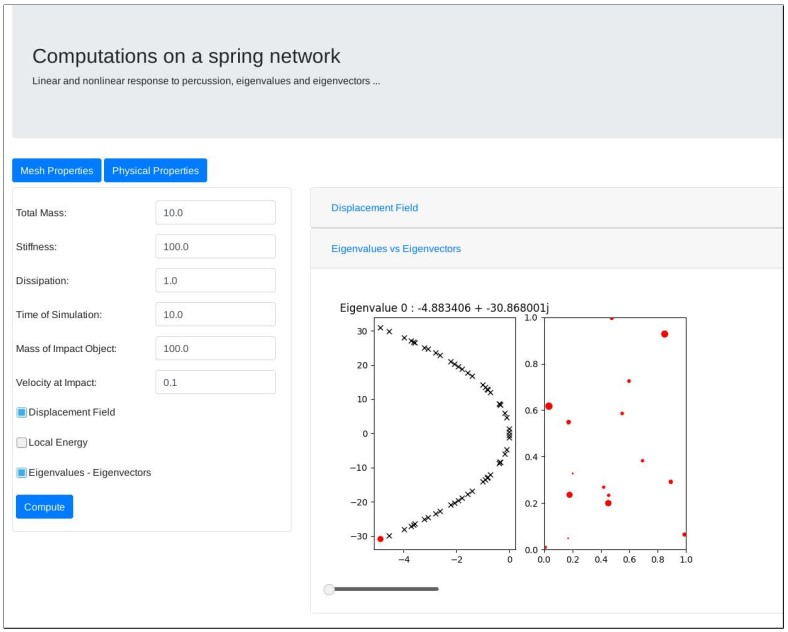
\includegraphics[width=0.85\textwidth]{ClientWebBal.jpg}
    \caption{Client web \texttt{springslattice-web.py} développé dans \parencite[p.197]{balasoiu2020halthesis}.}
    \label{fig:clientwebbal}
\end{figure}




\subsection{Nouveaux travaux sur la percussion}



Les floes de glace $\Omega_k$ et $\Omega_l$ sont modélisés par des systèmes masse-ressort (à grande raideur). Pour l'instant, nous considérons une modélisation simplifiée qui assimile un floe à un système de (trois) masses reliés par des ressorts (de constante de raideur $k$), et par des dispositifs visqueux de constante $\mu$.
Nous désignerons par $n$ le nombre total de n\oe{}uds du floe $\Omega_k$, chaque n\oe{}ud ayant pour masse $m$. De façon similaire, on définit les constantes $k'$, $\mu'$, $n'$, $m'$ pour le floe $\Omega_l$. Les positions des n\oe{}uds de $\Omega_k$ seront notées $(\bvec q_i)_{0\leq i\leq n-1}$, tandis que celles de $\Omega_l$ seront notées $(\bvec p_i)_{0 \leq i\leq n'-1}$ (voir \cref{fig:contactmanuel}). 

\begin{figure}[!h]
    \centering
    % 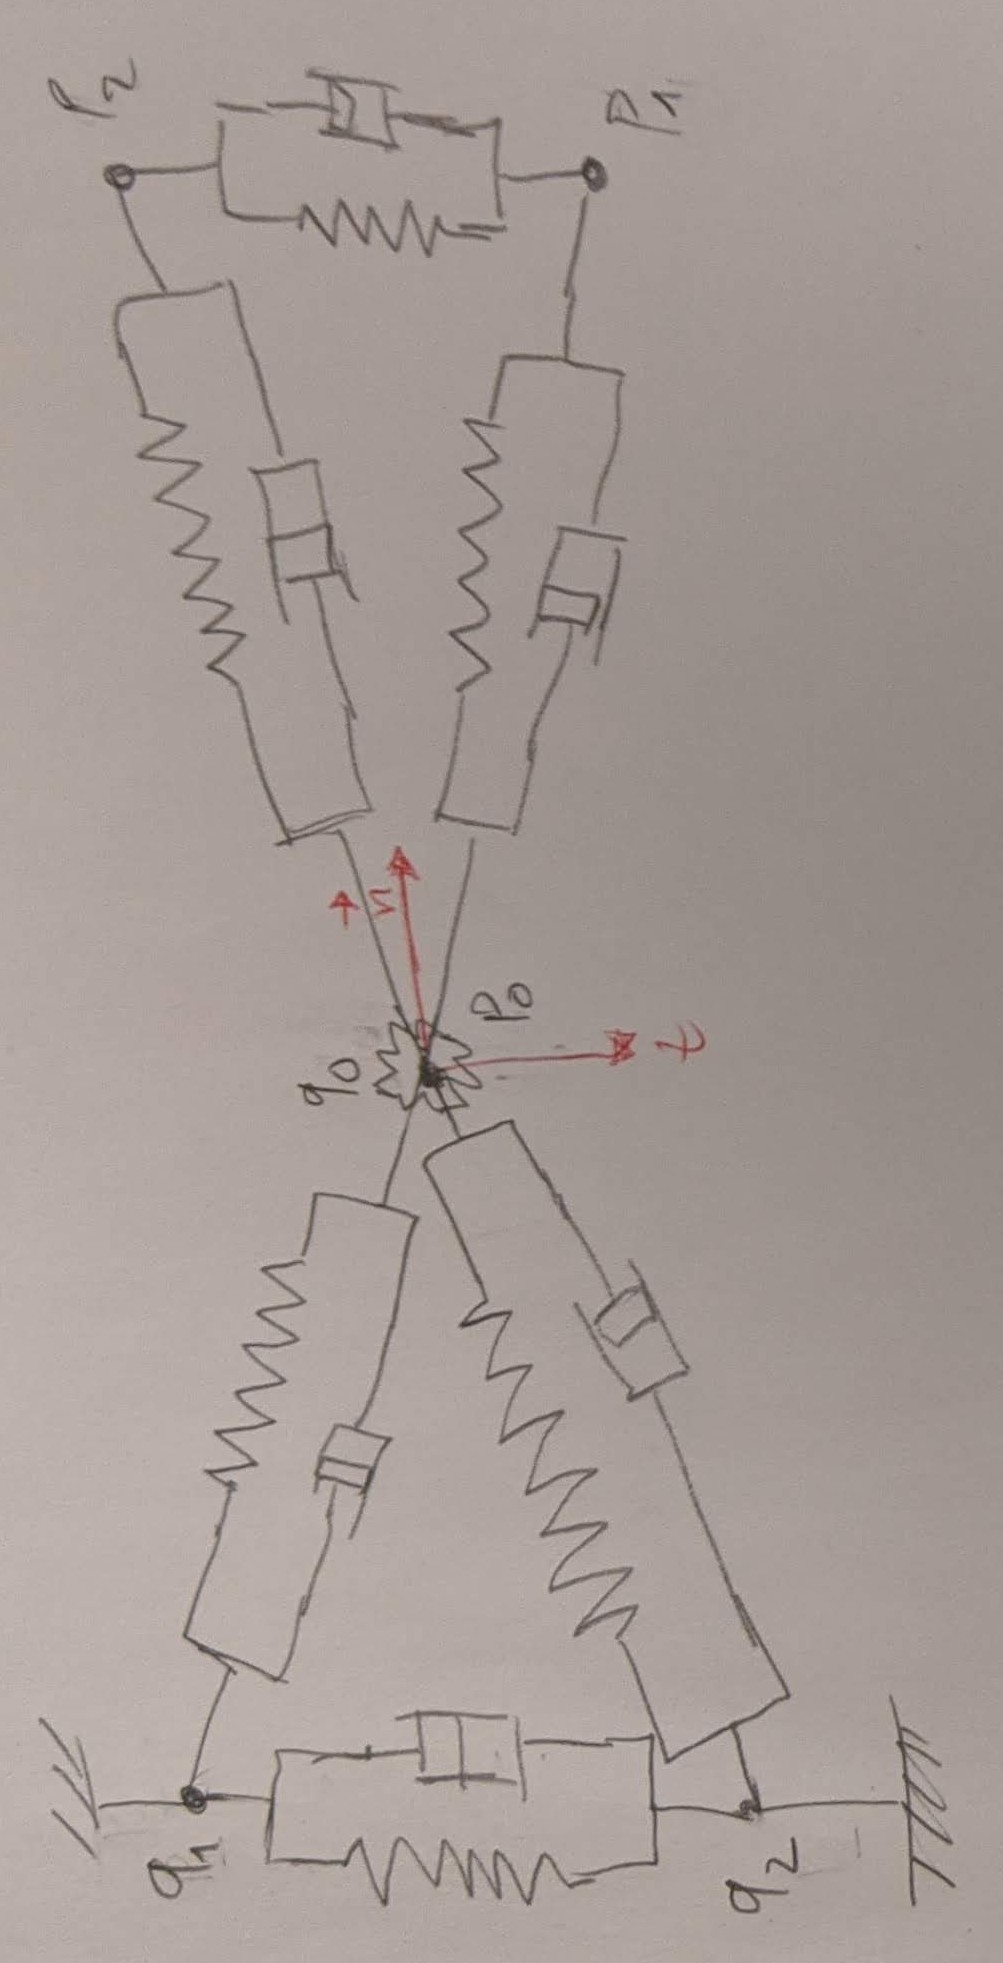
\includegraphics[width=0.3\textwidth, angle=-90]{ContactManuel.jpg}
    \frame{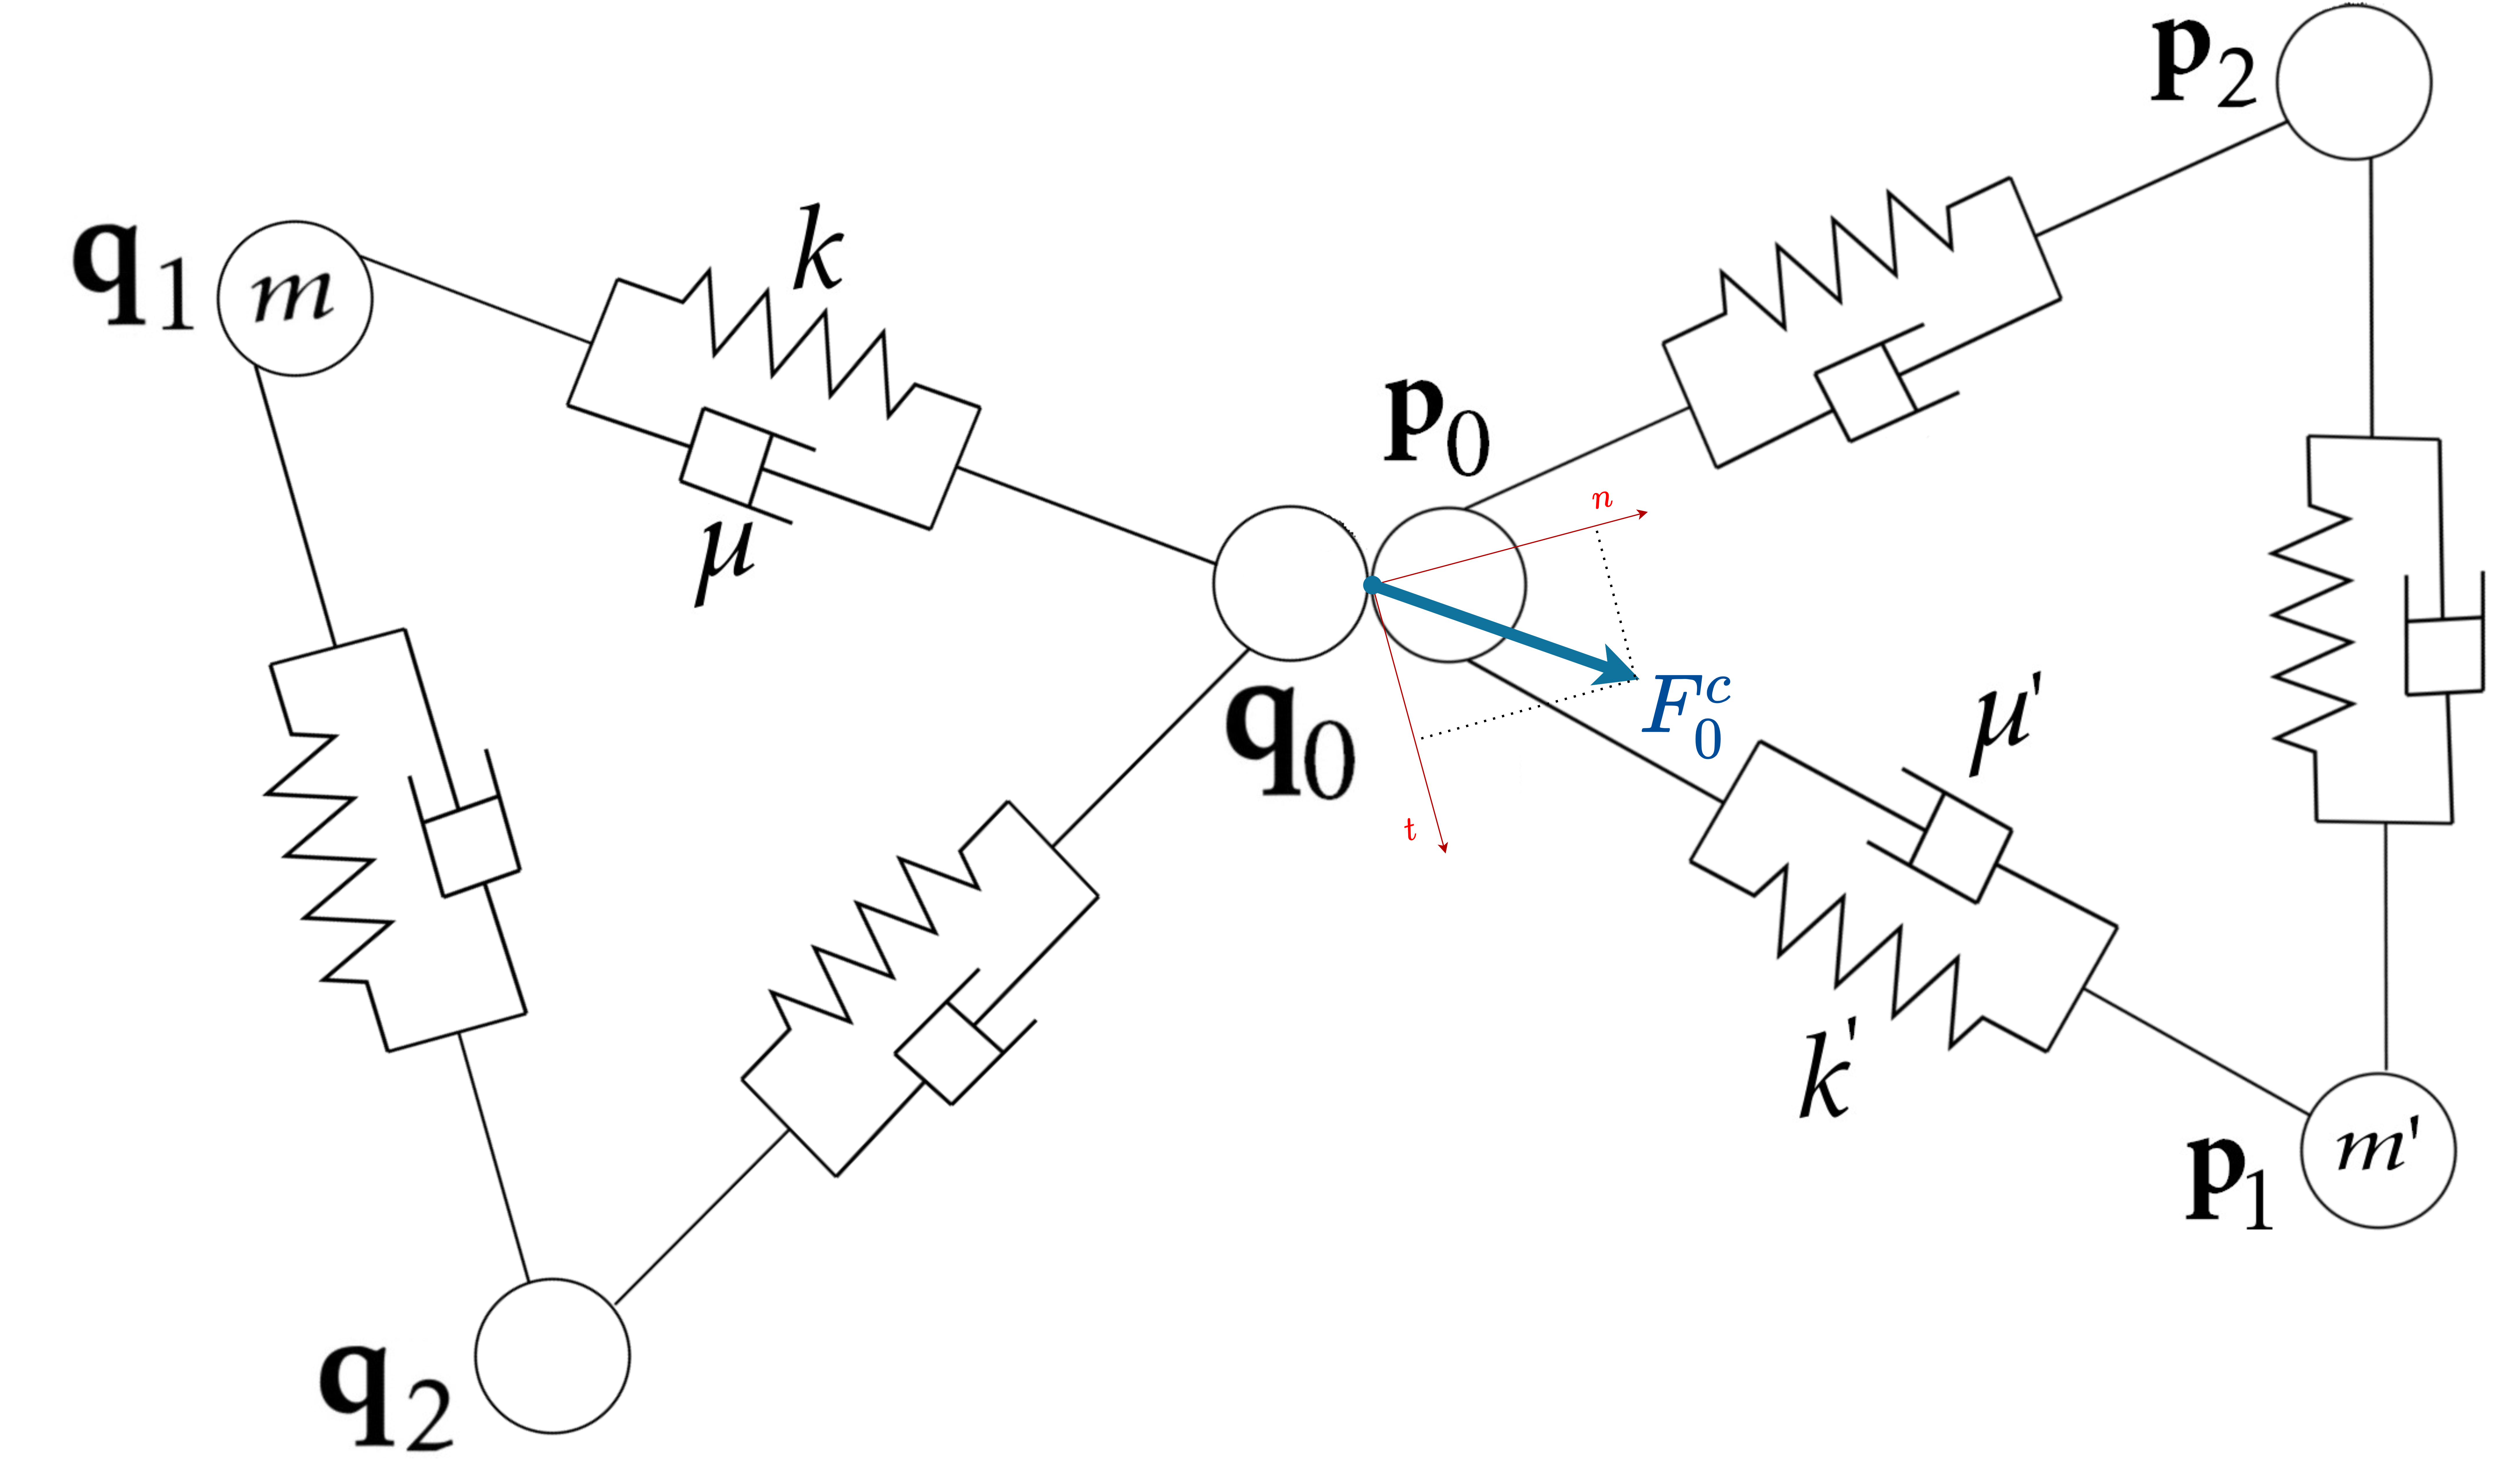
\includegraphics[width=0.65\textwidth]{Percussion2DNew.png}}
    \caption{Contact entre deux floes aux points $\bvec{q}_0$ et $\bvec{p}_0$ respectivement.}
    \label{fig:contactmanuel}
\end{figure}

\noindent On définit la longueur du ressort à vide $L_{0j}$ entre le n\oe{}ud $\bvec{q}_0$ et le n\oe{}ud $\bvec{q}_j$, et le vecteur unitaire $\bvec{u}_{0j}$ (orienté de $\bvec{q}_0$ vers $\bvec{q}_j$)\footnote{Notons que ces définitions sont naturellement adaptables si nous remplaçons le n\oe{}ud $\bvec{q}_0$ par un n\oe{}ud $(\bvec{q}_i)_{0 \leq i \leq n-1}$.}. On définit aussi la matrice de connectivité $C$:
\begin{align*}
    \forall \, 0 \leq i < j \leq n-1, \quad C_{ij} = C_{ji} = \begin{dcases}
    1 \text{ si } \bvec{q}_i \text{ est voisin de } \bvec{q}_j \,, \\
    0 \text{ sinon}.
\end{dcases}
\end{align*}
\noindent Comme présenté dans les travaux \parencite[p.186]{balasoiu2020halthesis}, le système différentiel qui modélise la percussion s’écrit comme le couplage de deux sous-systèmes. Le premier, dit système intérieur (SI), est à évolution rapide et modélise la propagation des ondes élastiques dans le système masse-ressort. Ici, nous dérivons facilement et réutilisons le SI comme présenté par \citeauthor{balasoiu2020halthesis}. Le second, dit système extérieur (SE), est à évolution lente et modélise la pénétration de l’objet percutant dans le système masse-ressorts percuté. Pour dériver le SE sur le floe $\Omega_k$, nous écrivons l'équation de Newton-Euler linéaire\footnote{La rotation du point matériel $\bvec q_0$ n'est pas prise en compte ici, d'où l'absence de l'équation de Newton-Euler angulaire.} au point de contact $\bvec q_0$:
\begin{align}  \label{eq:SE}
m \ddot{\bvec{q}}_0 = \bvec{F}_0 + \bvec{F}^c_0 \,,
\end{align}
où :
\begin{align}  \label{eq:F0}
    \bvec{F}_0 = \sum_{j=0}^{n-1}C_{0j} \left[  \underbrace{k \left( \Vert \bvec{q}_j - \bvec{q}_0 \Vert - L_{0j} \right) \bvec{u}_{0j}}_{\text{Force de rappel}} - \underbrace{\mu \left\langle \bvec{\dot{q}}_j - \bvec{\dot{q}}_0\,, \bvec{u}_{0j}  \right\rangle  \bvec{u}_{0j}}_{\text{Force de dissipation}}  \right] \,,
\end{align}
représente la somme des forces de réaction et de dissipation exercées par le ressort et le dispositif visqueux sur le n\oe{}ud $\bvec q_0$ ; et $\bvec{F}^c_0$ la force de contact durant la collision entre les deux particules. En supposant qu'il existe un repère de contact $\mathcal{R}^c = \{ q_0, \bvec{n}, \bvec{t} \}$ associé au floe $\Omega_k$ (voir \cref{fig:contactmanuel}), on peut écrire, pour $(\lambda, \beta) \in \Rdeux$ :
\begin{align}  \label{eq:F0c}
    \bvec{F}_0^c = \lambda \bvec{n} + \beta \bvec{t} \,.
\end{align}
Le système intérieur (SE) s'obtient facilement en combinant les équations \cref{eq:SE,eq:F0,eq:F0c}. Le système intérieur (SI) s'obtient lui (pour les autres n\oe{}uds du réseau) en y supprimant la force de contact. On obtient au final:
\begin{align} \tag{$E$} \label{eq:e}
\begin{dcases}
    m \ddot{\bvec{q}}_0 = \bvec{F}_0 + \bvec{F}^c_0  \,, &\qquad \text{(SE)} \\
    m \ddot{\bvec{q}}_i = \bvec{F}_i   \,, \quad \quad \quad \forall 1 \leq i \leq n-1 \,. &\qquad \text{(SI)}
\end{dcases}
\end{align}
En ce qui concerne le floe $\Omega_l$, nous procédons de façon similaire et appliquons la troisième loi de Newton (action-réaction) pour obtenir le système:
\begin{align} \tag{$E'$} \label{eq:eprime}
\begin{dcases}
    m' \ddot{\bvec{p}}_0 = \bvec{F}^{'}_0 - \bvec{F}^c_0  \,, &\qquad \text{(SE)} \\
    m' \ddot{\bvec{p}}_i = \bvec{F}^{'}_i   \,, \quad \quad \quad \forall 1 \leq i \leq n'-1 \,, &\qquad \text{(SI)}
\end{dcases}
\end{align}
où les $(\bvec{F}^{'}_i)_{0 \leq i \leq n'-1}$ sont définis de façon similaire à $\bvec{F}_0$ (voir \cref{eq:F0}):
\begin{align}
    \bvec{F}'_i = \sum_{j=i}^{n'-1}C_{ij} \left[ k' \left( \Vert \bvec{p}_j - \bvec{p}_i \Vert - L'_{ij} \right) \bvec{u'}_{ij} - \mu' \left\langle \bvec{\dot{p}}_j - \bvec{\dot{p}}_i\,, \bvec{u}'_{ij}  \right\rangle  \bvec{u}'_{ij}  \right] \,.
\end{align}

\noindent Ensuite, on additionne membre à membre les équations des systèmes extérieurs (SE) des \cref{eq:e,eq:eprime} pour éliminer la force de contact. On obtient:
\begin{align}
m \ddot{\bvec{q}}_0 + m' \ddot{\bvec{p}}_0 = \bvec{F}_0 + \bvec{F}^{'}_0 \,.
\end{align}
Remarquons que les positions relatives des n\oe{}uds $\bvec{q}_0$ et $\bvec{p}_0$ restent inchangées durant la collision. A l'instant initial, on note donc $\Delta_0 = \bvec{q}_0(0) - \bvec{p}_0(0)$, et $\bvec{\dot q}_0(0) = \bvec{\dot p}_0(0)$ ; idéalement, nous voudrions que:
\begin{align}
\forall t \in \mathbb{R}^+ \,, \quad \bvec{q}_0(t) - \bvec{p}_0(t) = \Delta_0\,.
\end{align}
Pour satisfaire cette condition, nous exhibons autant d'équations nécessaires pour que notre problème de percussion soit bien posé. Elles sont :
\begin{align} \tag{$\mathcal{P}$} \label{eq:problemeP}
\begin{dcases}
    (m+m') \ddot{\bvec{q}}_0  = \bvec{F}_0 + \bvec{F}^{'}_0  \,, &\qquad \text{(SE)} \\
    \ddot{\bvec{p}}_0 = \ddot{\bvec{q}}_0 \,, \quad \dot{\bvec{p}}_0 = \dot{\bvec{q}}_0 \,, \quad \bvec{p}_0 = \bvec{q}_0 - \Delta_0 \,, &\qquad \text{(SE)} \\
    m \ddot{\bvec{q}}_i = \bvec{F}_i   \,, \quad \quad \quad \forall 1 \leq i \leq n-1 \,. &\qquad \text{(SI)} \\
    m' \ddot{\bvec{p}}_i = \bvec{F}^{'}_i   \,, \quad \quad \quad \forall 1 \leq i \leq n'-1 \,, &\qquad \text{(SI)}
\end{dcases}
\end{align}

Quant à la visualisation des résultats, nous avons construit une interface web pour interagir avec le programme. À travers ce client, nous pouvons modifier tous les paramètres du problème et lancer des simulations. Un tel exemple se trouve à la \cref{fig:clientwebmoi}, et la simulation correspondante peut être visualisée via \href{https://seafile.unistra.fr/f/8ab67b150b724e9baf6b/}{ce lien}. 




%3----------------------------------------------------------------------------------------

\section{Code de calcul 2D}


L'algorithme de calcul 2D est largement inspiré des travaux de \citeauthor{balasoiu2020halthesis}. En effet, nous avons ajouté des modules Python au package \texttt{springslattice} qu'il à développé pour traiter les réseaux de ressorts. Ces nouveaux modules sont:
\begin{enumerate}
    \item \textbf{multimesh}: pour la création d'un réseau de ressort constitué de deux floes de glace en contact, qui nous servira de maillage (voir \cref{fig:percussion2d}).
    \item \textbf{multisolver}: pour la création du solveur 2D suivant l'\cref{eq:problemeP} pour simuler les n\oe{}uds d'un objet \texttt{multimesh}. Une fois les calculs faits dans la fonction \texttt{Fhom}, nous les vérifions à l'aide d'un schéma symplectique.
    \item \textbf{percussion-cli}: pour l'exécution des simulations avec des paramètres donnés en ligne de commande (ou ceux insérer par défaut).
    \item \textbf{percussion-web}: pour l'exécution des simulations avec des paramètres donnés dans une interface web. Ici, on peut en plus observer les vecteurs et les valeurs propres (toutes négatives) du système (voir \cref{fig:clientwebmoi}).
\end{enumerate}


Nous présentons à la \cref{fig:readme2d} le fichier README du dépôt \href{https://framagit.org/RaK/SimuRessorts}{springslattice} sur \texttt{Framagit} créer par Balasoiu dans ses travaux, et maintenu et amélioré par nous durant ce stage. Tout comme le dépôt principal \href{https://github.com/desmond-rn/ice-floes}{ice-floes} sur \texttt{GitHub}, ce dépôt secondaire est privé.



\begin{figure}[H]
    \centering
    \frame{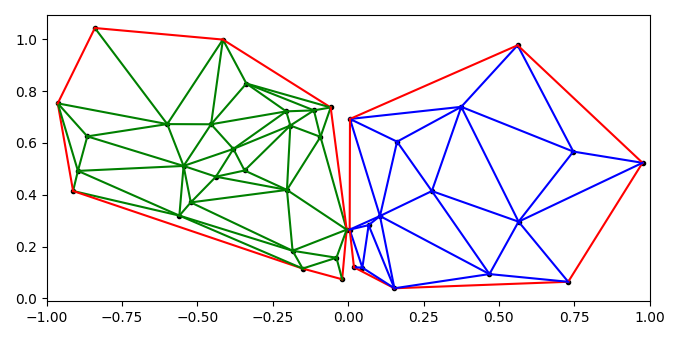
\includegraphics[width=0.65\textwidth]{Percussion2D}}
    \caption{Exemple de maillage 2D pour la percussion.}
    \label{fig:percussion2d}
\end{figure}


\begin{figure}[H]
    \centering
    \frame{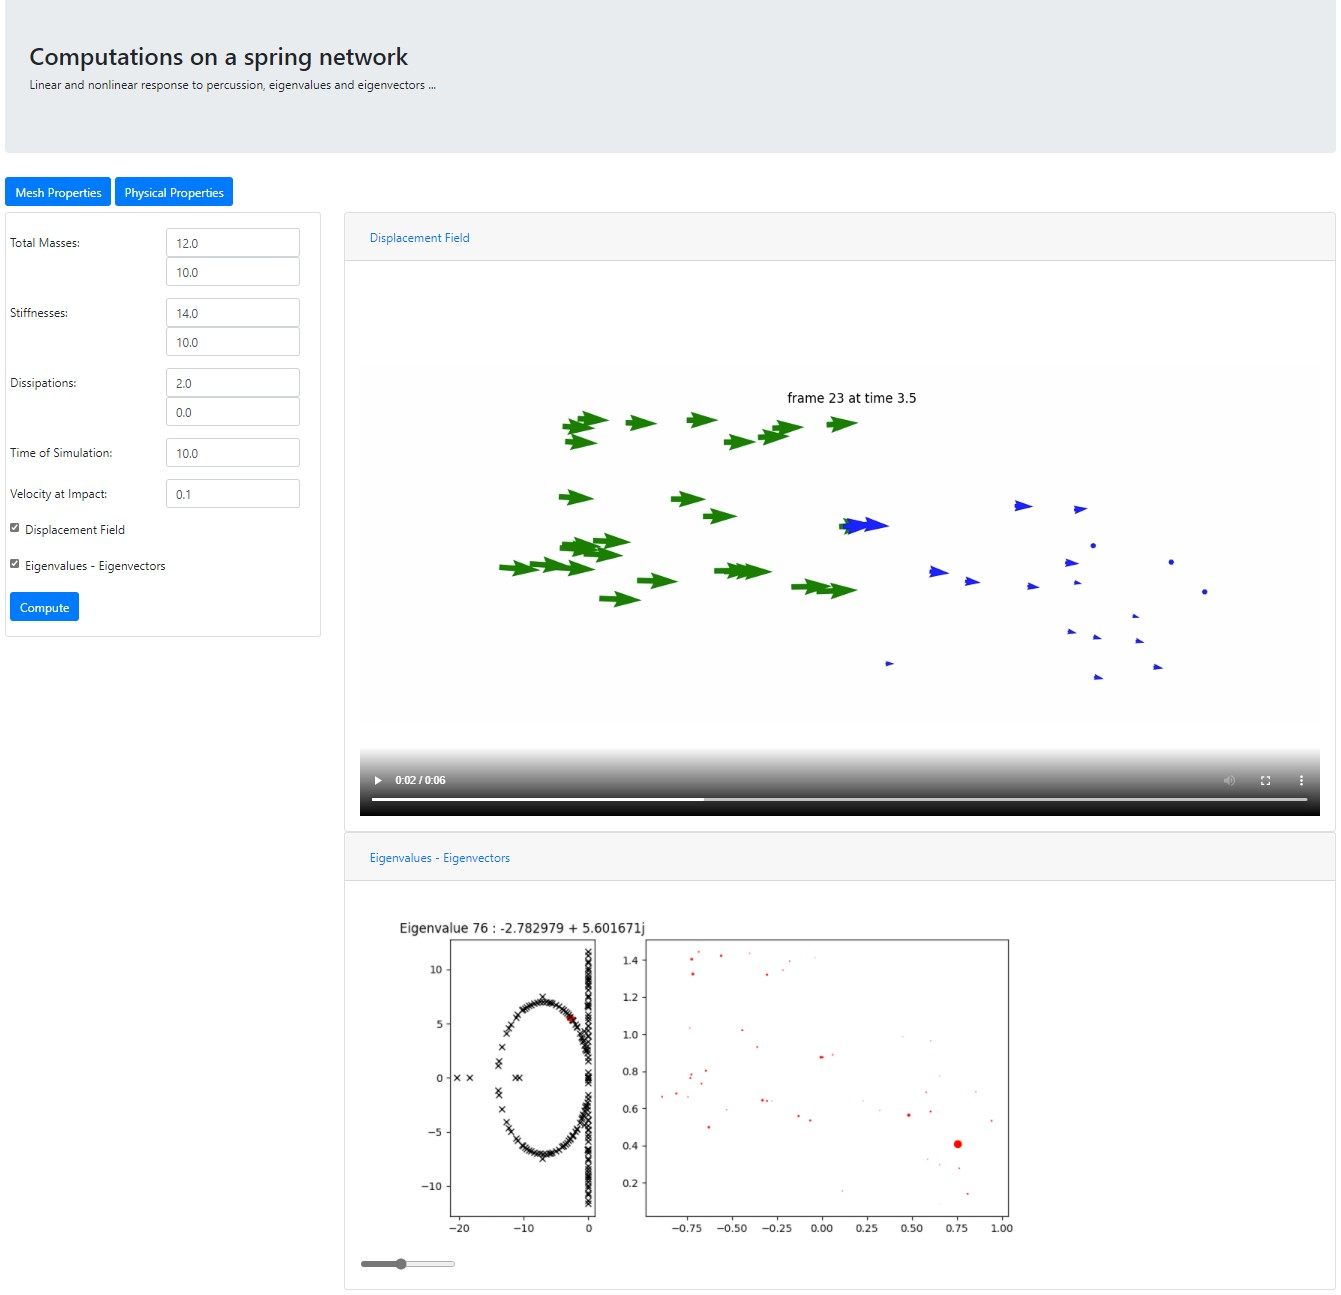
\includegraphics[width=0.93\textwidth]{ClientWebMoi.jpg}}
    \caption{Client web développé durant le stage pour les percussions 2D. Comparativement à la \cref{fig:clientwebbal}, on constate la présence de plus de champ, surtout ceux pour préciser les paramètres du second floe entrant en collision.}
    \label{fig:clientwebmoi}
\end{figure}



\begin{figure}[!h]
    \centering
    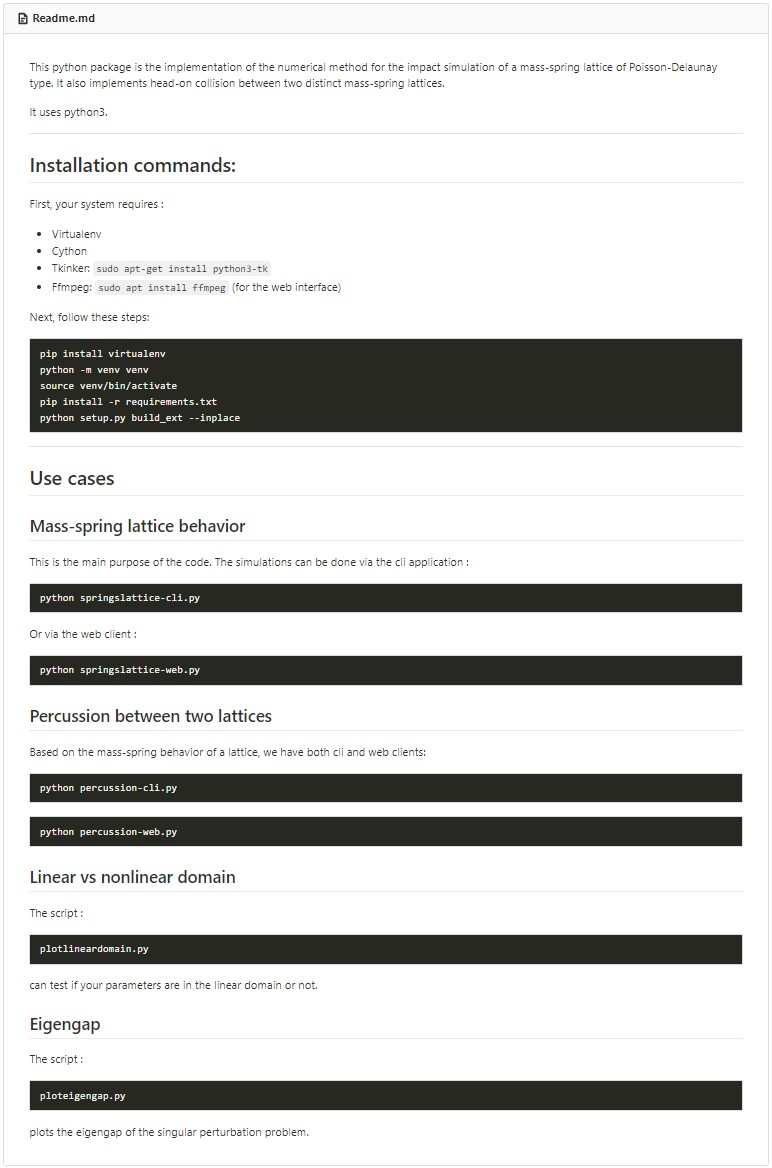
\includegraphics[width=0.85\textwidth]{ReadmeRepoSpringsLattice.jpg}
    \caption{Appercu du dépot secondaire \href{https://framagit.org/RaK/SimuRessorts/-/tree/master}{springslattice} maintenu et amélioré durant le stage.}
    \label{fig:readme2d}
\end{figure}


%4----------------------------------------------------------------------------------------

\section{Résumé des résultats obtenus}

Bien que le modèle de fracture 1D soit facilement adaptable aux calculs 2D, nous ne l'avons pas fait faute de temps. En résumé, nous avons fait ceci:
\begin{itemize}
    \item Modélisation du déplacement des n\oe{}uds d'un floe de glace 2D soumis à aucune force sur son bord;
    \item Modélisation de la collision (élastique) de deux floes de glace. Vu que le temps de la collision est connu (voir \parencite{rabatel2015thesis}), nous pouvons étendre ces travaux à la collision avec séparation des masses, comme nous l'avons fait en 1D;
    \item Création d'un interface web pour introduire les paramètres et obtenir les résultats d'une simulation. 
\end{itemize}

Les résultats obtenus en 2D sont prometteurs, tout comme ceux obtenus en 1D. Ils ont été obtenu pendant un stage qui a demandé un discipline et une encadrement de taille. Au bout de ce travail, j'ai vu mes compétences dans divers domaines considérablement améliorées.
